\section{Stato dei Requisiti Funzionali}

\subsection{Stato per requisito}
\begin{longtable}{|p{2.5cm}|p{9cm}|p{3cm}|}
\hline
\textbf{Codice} & \textbf{Descrizione} & \textbf{Stato} \\
\hline
\endhead

RF1-OB & L'Utente deve potersi autenticare presso il Sistema & Soddisfatto \\
\hline
RF2-OB & L'Utente deve inserire il proprio username per autenticarsi presso il Sistema & Soddisfatto \\
\hline
RF3-OB & L'Utente deve inserire la propria password per autenticarsi presso il Sistema & Soddisfatto \\
\hline
RF4-OB & L'Utente deve ricevere un errore se l'username non è registrato nel Sistema o la password non è corretta per l'Utente inserito & Soddisfatto \\
\hline
RF5-OB & L'Utente deve potersi autenticare presso il Sistema e impostare una nuova password & Soddisfatto \\
\hline
RF6-OB & L'Utente deve inserire la password temporanea che gli è stata fornita dall'amministratore per autenticarsi presso il Sistema e impostare una nuova password & Soddisfatto \\
\hline
RF7-OB & L'Utente deve inserire la nuova password per registrarsi presso il Sistema & Soddisfatto \\
\hline
RF8-OB & L'Utente deve ricevere un errore se l'username non è registrato nel Sistema o la password temporanea non è corretta per l'Utente inserito & Soddisfatto \\
\hline
RF9-OB & L'Utente deve ricevere un errore se la nuova password è uguale alla password temporanea & Soddisfatto \\
\hline
RF10-OB & L'Utente deve ricevere un errore se la nuova password non rispetta i criteri richiesti & Soddisfatto \\
\hline
RF11-OB & L'Amministratore deve poter visualizzare se un account MyVimar è configurato nel Sistema & Soddisfatto \\
\hline
RF12-OB & L'Amministratore visualizzando l'account MyVimar collegato deve visualizzare l'email dell'account & Soddisfatto \\
\hline
RF13-OB & L'Amministratore deve poter collegare un account MyVimar nel Sistema & Soddisfatto \\
\hline
RF14-OB & L'Amministratore deve poter rimuovere un account MyVimar dal Sistema & Soddisfatto \\
\hline
RF15-DE & L'Amministratore deve poter visualizzare l'elenco degli utenti del Sistema & Soddisfatto \\
\hline
RF16-OB & L'Amministratore visualizzando l'elenco degli utenti del sistema deve visualizzare un utente del Sistema nel dettaglio & Soddisfatto \\
\hline
RF17-OB & L'Amministratore visualizzando un utente del sistema nel dettaglio deve visualizzare il nome & Soddisfatto \\
\hline
RF18-OB & L'Amministratore visualizzando un utente del sistema nel dettaglio deve visualizzare il cognome & Soddisfatto \\
\hline
RF19-OB & L'Amministratore visualizzando un utente del sistema nel dettaglio deve visualizzare l'username & Soddisfatto \\
\hline
RF20-DE & L'Amministratore deve poter creare un utente Operatore Sanitario & Soddisfatto \\
\hline
RF21-DE & L'Amministratore deve inserire il nome dell'Operatore Sanitario per creare un utente Operatore Sanitario & Soddisfatto \\
\hline
RF22-DE & L'Amministratore deve inserire il cognome dell'Operatore Sanitario per creare un utente Operatore Sanitario & Soddisfatto \\
\hline
RF23-DE & L'Amministratore deve inserire un username per creare un utente Operatore Sanitario & Soddisfatto \\
\hline
RF24-DE & L'Amministratore deve generare la password temporanea per creare un utente Operatore Sanitario & Soddisfatto \\
\hline
RF25-DE & L'Amministratore deve ricevere un errore se l'username è già in uso & Soddisfatto \\
\hline
RF26-DE & L'Amministratore deve poter eliminare un utente Operatore Sanitario & Soddisfatto \\
\hline
RF27-OB & L'Amministratore deve poter visualizzare tutti i reparti del Sistema & Soddisfatto \\
\hline
RF28-OB & L'Amministratore deve poter visualizzare un reparto del Sistema nel dettaglio & Soddisfatto \\
\hline
RF29-OB & L'Amministratore visualizzando un reparto del Sistema deve poter visualizzare il nome del reparto & Soddisfatto \\
\hline
RF30-OB & L'Amministratore deve poter creare un nuovo reparto nel Sistema & Soddisfatto \\
\hline
RF31-OB & L'Amministratore deve inserire il nome del nuovo reparto per crearlo nel Sistema & Soddisfatto \\
\hline
RF32-OB & L'Amministratore deve ricevere un errore se il nome del nuovo reparto è già in uso & Soddisfatto \\
\hline
RF33-OB & L'Amministratore deve poter modificare il nome di un reparto del Sistema & Soddisfatto \\
\hline
RF34-OB & L'Amministratore deve poter eliminare un reparto del Sistema & Soddisfatto \\
\hline
RF35-OB & L'Amministratore deve poter assegnare un reparto a un utente Operatore Sanitario & Soddisfatto \\
\hline
RF36-OB & L'Amministratore deve selezionare un utente Operatore Sanitario per assegnare a un utente Operatore Sanitario un reparto & Soddisfatto \\
\hline
RF37-OB & L'Amministratore deve selezionare un reparto per assegnare un reparto a un utente Operatore Sanitario & Soddisfatto \\
\hline
RF38-OB & L'Amministratore deve poter eliminare l'assegnazione utente Operatore Sanitario -- reparto & Soddisfatto \\
\hline
RF39-OB & L'Amministratore deve poter assegnare un reparto a un appartamento & Soddisfatto \\
\hline
RF40-OB & L'Amministratore deve selezionare un appartamento per assegnare a un appartamento un reparto & Soddisfatto \\
\hline
RF41-OB & L'Amministratore deve selezionare un reparto per assegnare un reparto a un appartamento & Soddisfatto \\
\hline
RF42-OB & L'Amministratore deve poter eliminare l'assegnazione appartamento -- reparto & Soddisfatto \\
\hline
RF43-OB & L'Utente deve poter visualizzare una dashboard che rappresenta lo stato del Sistema & Soddisfatto \\
\hline
RF44-OB & L'Utente visualizzando la dashboard deve poter visualizzare un modulo gestione allarmi & Soddisfatto \\
\hline
RF45-OB & L'Utente visualizzando il modulo gestione allarmi deve poter visualizzare ogni singolo allarme & Soddisfatto \\
\hline
RF46-OB & L'Utente visualizzando un singolo allarme deve poter visualizzare il segnale di pericolo & Soddisfatto \\
\hline
RF47-OB & L'Utente visualizzando un singolo allarme deve poter visualizzare il nome & Soddisfatto \\
\hline
RF48-OB & L'Utente visualizzando un singolo allarme deve poter visualizzare il tempo trascorso dallo scatto dell'allarme & Soddisfatto \\
\hline
RF49-OB & L'Utente visualizzando la dashboard deve poter visualizzare un modulo statistiche allarmi & Soddisfatto \\
\hline
RF50-OB & L'Utente visualizzando il modulo statistiche allarmi deve poter visualizzare il numero di allarmi risolti & Soddisfatto \\
\hline
RF51-OB & L'Utente visualizzando il modulo statistiche allarmi deve poter visualizzare il numero di allarmi attivi & Soddisfatto \\
\hline
RF52-OB & L'Utente visualizzando la dashboard deve poter visualizzare un modulo informazioni Utente & Soddisfatto \\
\hline
RF53-OB & L'Utente visualizzando il modulo informazioni Utente deve poter visualizzare il nome Utente & Soddisfatto \\
\hline
RF54-OB & L'Utente visualizzando il modulo informazioni Utente deve poter visualizzare il cognome Utente & Soddisfatto \\
\hline
RF55-OB & L'Utente visualizzando la dashboard deve poter visualizzare un modulo analisi clima & Soddisfatto \\
\hline
RF56-OB & L'Utente visualizzando la dashboard deve poter visualizzare un modulo analisi consumi & Soddisfatto \\
\hline
RF57-OB & L'Utente visualizzando la dashboard deve poter visualizzare un modulo analisi presenze & Soddisfatto \\
\hline
RF58-DE & L'Amministratore deve poter aggiungere alla visualizzazione della dashboard un modulo tra i seguenti: statistiche allarmi; informazioni Utente; analisi clima; analisi consumi & Soddisfatto \\
\hline
RF59-DE & L'Amministratore deve poter rimuovere dalla visualizzazione della dashboard un modulo tra i seguenti: statistiche allarmi; informazioni Utente; analisi clima; analisi consumi & Soddisfatto \\
\hline
RF60-OB & L'Utente deve poter risolvere un allarme & Soddisfatto \\
\hline
RF61-OB & L'Utente deve poter visualizzare le analytics & Soddisfatto \\
\hline
RF62-OB & L'Utente visualizzando le analytics deve visualizzare l'elenco dei suggerimenti risparmio energetico & Soddisfatto \\
\hline
RF63-OB & L'Utente visualizzando l'elenco dei suggerimenti risparmio energetico deve visualizzare un suggerimento risparmio energetico & Soddisfatto \\
\hline
RF64-OB & L'Utente visualizzando le analytics deve visualizzare il grafico dedicato al consumo energetico & Soddisfatto \\
\hline
RF65-OB & L'Utente visualizzando le analytics deve visualizzare il grafico dedicato alle anomalie dell'impianto & Soddisfatto \\
\hline
RF66-OB & L'Utente visualizzando le analytics deve visualizzare il grafico relativo al rilevamento di presenza & Soddisfatto \\
\hline
RF67-OB & L'Utente visualizzando le analytics deve visualizzare il grafico relativo alla presenza prolungata nello stesso ambiente & Soddisfatto \\
\hline
RF68-OB & L'Utente visualizzando le analytics deve visualizzare il grafico relativo alle variazioni di temperatura & Soddisfatto \\
\hline
RF69-OB & L'Utente visualizzando le analytics deve visualizzare il grafico relativo agli allarmi inviati e risolti & Soddisfatto \\
\hline
RF70-OP & L'Utente visualizzando le analytics deve visualizzare il grafico relativo alla frequenza degli allarmi & Soddisfatto \\
\hline
RF71-OP & L'Utente visualizzando le analytics deve visualizzare il grafico relativo alla frequenza delle cadute & Soddisfatto \\
\hline
RF72-OB & L'Utente deve poter visualizzare un appartamento del Sistema & Soddisfatto \\
\hline
RF73-OB & L'Utente visualizzando un appartamento del Sistema deve visualizzare il nome dell'appartamento & Soddisfatto \\
\hline
RF74-OP & L'Utente visualizzando un appartamento del Sistema deve visualizzare la mappa degli allarmi dell'appartamento & Soddisfatto \\
\hline
RF75-OB & L'Utente visualizzando un appartamento del Sistema deve visualizzare le stanze dell'appartamento & Soddisfatto \\
\hline
RF76-OB & L'Utente deve visualizzare una stanza nel dettaglio & Soddisfatto \\
\hline
RF77-OB & L'Utente visualizzando una stanza deve visualizzare il nome della stanza & Soddisfatto \\
\hline
RF78-OB & L'Utente visualizzando una stanza deve visualizzare l'elenco dei dispositivi della stanza & Soddisfatto \\
\hline
RF79-OB & L'Utente visualizzando l'elenco dei dispositivi deve visualizzare un singolo dispositivo di tipo: termostato; sensore di caduta; sensore di presenza; punto luce; pulsante di allarme; porta di ingresso; tapparella & Soddisfatto \\
\hline
RF80-OB & L'Utente visualizzando un dispositivo deve vedere il nome & Soddisfatto \\
\hline
RF81-OB & L'Utente visualizzando un dispositivo deve vedere lo stato & Soddisfatto \\
\hline
RF82-OP & L'Utente visualizzando un dispositivo deve vedere le azioni eseguibili & Soddisfatto \\
\hline
RF83-OP & L'Amministratore deve poter abilitare un appartamento nel Sistema & Non soddisfatto \\
\hline
RF84-OP & L'Amministratore deve poter disabilitare un appartamento nel Sistema & Non soddisfatto \\
\hline
RF85-OB & L'Amministratore deve poter creare un allarme nel Sistema & Soddisfatto \\
\hline
RF86-OB & L'Amministratore deve selezionare l'appartamento per creare un allarme nel Sistema & Soddisfatto \\
\hline
RF87-OB & L'Amministratore deve selezionare il sensore per creare un allarme nel Sistema & Soddisfatto \\
\hline
RF88-OB & L'Amministratore deve selezionare il livello di priorità tra: priorità 1 (bianco); priorità 2 (verde); priorità 3 (arancione); priorità 4 (rosso) per creare un allarme nel Sistema & Soddisfatto \\
\hline
RF89-OB & L'Amministratore deve selezionare una soglia di intervento per creare un allarme nel Sistema & Soddisfatto \\
\hline
RF90-OB & L'Amministratore deve selezionare un orario di attivazione per creare un allarme nel Sistema & Soddisfatto \\
\hline
RF91-OB & L'Amministratore deve selezionare un orario di disattivazione per creare un allarme nel Sistema & Soddisfatto \\
\hline
RF92-OB & L'Amministratore deve ricevere un errore se non ha selezionato alcun sensore & Soddisfatto \\
\hline
RF93-OB & L'Amministratore deve ricevere un errore se non ha selezionato alcun livello di priorità & Soddisfatto \\
\hline
RF94-OB & L'Amministratore deve ricevere un errore se non ha selezionato alcuna soglia di intervento & Soddisfatto \\
\hline
RF95-OB & L'Amministratore deve poter modificare la priorità di un allarme del Sistema & Soddisfatto \\
\hline
RF96-OB & L'Amministratore deve poter modificare la soglia d'intervento di un allarme del Sistema & Soddisfatto \\
\hline
RF97-OB & L'Amministratore deve poter modificare l'orario di attivazione di un allarme del Sistema & Soddisfatto \\
\hline
RF98-OB & L'Amministratore deve poter modificare l'orario di disattivazione di un allarme del Sistema & Soddisfatto \\
\hline
RF99-OB & L'Amministratore deve poter abilitare un allarme del Sistema & Soddisfatto \\
\hline
RF100-OB & L'Amministratore deve poter disabilitare un allarme del Sistema & Soddisfatto \\
\hline
RF101-OB & L'Amministratore deve poter eliminare un allarme nel Sistema & Soddisfatto \\
\hline
RF102-OP & L'Utente deve poter visualizzare le notifiche inviate dal Sistema & Soddisfatto \\
\hline
RF103-OP & L'Utente visualizzando le notifiche deve poter visualizzare una notifica nel dettaglio & Soddisfatto \\
\hline
RF104-OP & L'Utente visualizzando una notifica deve poter visualizzare il titolo della notifica & Soddisfatto \\
\hline
RF105-OP & L'Utente visualizzando una notifica deve poter visualizzare il tempo trascorso dall'invio della notifica & Soddisfatto \\
\hline
\end{longtable}

\subsection{Grafici riassuntivi}
A seguire vengono presentati i grafici riassuntivi del soddisfacimento dei requisiti funzionali, 
suddivisi per tipologia di classificazione: obbligatori (OB), desiderabili (DE) e opzionali (OP). 
Per ciascuna categoria viene mostrata la percentuale di requisiti soddisfatti rispetto al totale 
previsto, al fine di fornire una visione immediata e sintetica del grado di completamento del 
Sistema rispetto a quanto definito nell'Analisi dei Requisiti.

\begin{figure}[H]
    \centering
    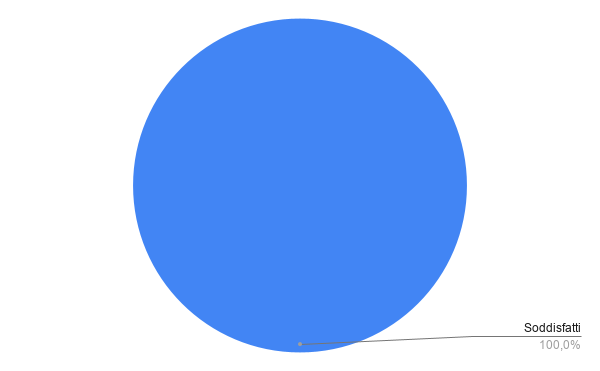
\includegraphics[width=0.6\textwidth]{./img/requisiti_ob.png}
    \caption{Percentuale di Requisiti Obbligatori Soddisfatti rispetto al totale}
\end{figure}

\begin{figure}[H]
    \centering
    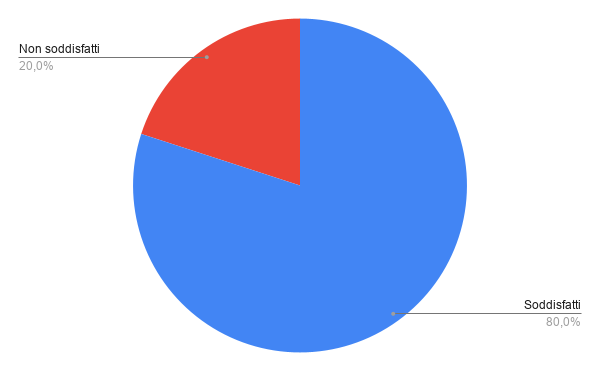
\includegraphics[width=0.6\textwidth]{./img/requisiti_op.png}
    \caption{Percentuale di Requisiti Opzionali Soddisfatti rispetto al totale}
\end{figure}

\begin{figure}[H]
    \centering
    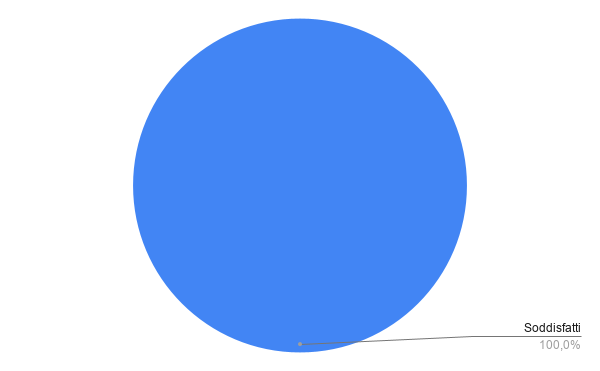
\includegraphics[width=0.6\textwidth]{./img/requisiti_des.png}
    \caption{Percentuale di Requisiti Desiderabili Soddisfatti rispetto al totale}
\end{figure}